% =====================================================================
%  第 6 章 §6.6 中段（原书 p.339–352 / PDF 349–362）—— ch06d2
%  续写；不写章标题、不写 §6.6 标题（已在 ch06d.tex 中）
% =====================================================================

% [原文 p.339]
Becker–Becker–Strominger [38] 研究了膜（brane）保持超对称性与 $\kappa$ 对称性（kappa symmetry）的条件\footnote{这些后面不用，故不说明。}，发现了特殊拉格朗日子流形这一条件。设 $M$ 为复 $n$ 维 Calabi–Yau 流形。（以下暂时不考虑 $B$ 场。即考虑（实）辛形式 $\omega$（凯勒形式）。）$M$ 上有全纯 $n$ 形式 $\Omega$。把 $\Omega$ 正规化，使各点的范数为 $1$。（由于 $\Omega\wedge\bar\Omega$ 是调和 $2n$ 形式，$\Omega$ 的范数不依赖于点。）

\begin{definition}{6.186}
  $n$ 维子流形 $L\subset M$ 称为\textbf{特殊拉格朗日子流形}（special Lagrangian submanifold），是指 $\Omega$ 在 $L$ 上的限制是 $L$ 的（关于诱导黎曼度量的）体积元素。
\end{definition}

\begin{lemma*}{6.187}
  特殊拉格朗日子流形是拉格朗日子流形。
\end{lemma*}
\begin{proof}
  设 $e_1,\dots,e_n$ 为 $T_pL$ 的正交基。由 $\Omega$ 是 $L$ 的体积元素，
  \[
    (\Omega\wedge\bar\Omega)(e_1\wedge Je_1\wedge\dots\wedge e_n\wedge Je_n)=\pm1.
  \]
  另一方面，$\Omega\wedge\bar\Omega$ 是 $M$ 的体积元素。因此 $Je_i$ 与 $T_pL$ 正交。即 $\omega(e_i,e_j)=\pm g_M(e_i,Je_j)=0$。
\end{proof}
% [Tutor Note: 特殊拉格朗日条件是比拉格朗日条件更强的要求：拉格朗日只要求 $\omega|_L=0$，而这里还要求 $\Omega$ 的辐角在 $L$ 上为常数（此处已把 $\Omega$ 正规化成模 1，故条件化为 $\Omega|_L$ 为实体积元素）。判断“特殊”时看的是 $\Omega$，不是 $\omega$。]

$\Omega$ 是校准（calibration）（注 2.84），特殊拉格朗日子流形是被校准的子流形。特别地，是极小子流形。

\begin{definition}{6.188}
  记 $\mathcal{LAG}_{sp}(M)$ 为 $M$ 的特殊拉格朗日子流形 $L$ 与其上的平坦复线丛 $\mathcal L$ 的组 $(L,\mathcal L)$ 的全体。
\end{definition}

Strominger–Yau–Zaslow [350] 发现：若 $\mathcal{LAG}_{sp}(M)$ 成为 $M$ 的镜像 $M^\dagger$ 上的凝聚层的模空间，则可得到从 $M$ 构造 $M^\dagger$ 的方法。他们的想法如下。设 $M^\dagger$ 为复流形。$p\in M^\dagger$ 如下确定 $M^\dagger$ 上的层 $\mathcal S_p$。

% [原文 p.340]
\begin{equation*}
  \mathcal S_p(U)=
  \begin{cases}
    \C, & p\in U \text{ 时},\\
    0, & p\notin U \text{ 时}.
  \end{cases}
\end{equation*}
$\mathcal S_p$ 称为\textbf{点层}（摩天层，skyscraper sheaf）。点层的模空间就是 $M^\dagger$ 本身，这是显然的。因此，若猜想 6.182 成立，则 $\mathcal{LAG}_{sp}(M)$ 必须包含 $M^\dagger$。Strominger–Yau–Zaslow 更准确地提出了以下的构造。

\begin{definition}{6.189}
  $\pi:M\to N$ 称为\textbf{特殊拉格朗日纤维丛}（special Lagrangian fiber bundle），是指存在余维数 $2$ 的子流形 $S(N)\subset N$，使对 $p\in N-S(N)$，$\pi^{-1}(p)$ 是特殊拉格朗日子流形，且 $\pi^{-1}(N-S(N))\to N-S(N)$ 是纤维丛。
\end{definition}

\begin{remark}{6.190}
  这个定义是暂定的。严格说来，还需要关于 $S(N)$ 上发生什么的条件。
\end{remark}

\begin{remark}{6.191}
  由定理 4.63，对 $p\in N-S(N)$，$\pi^{-1}(p)$ 是环面。
\end{remark}

\begin{example}{6.192}
  例 4.70，即取椭圆型 K3 曲面使其纤维成为拉格朗日子流形的复结构，是特殊拉格朗日纤维丛。
\end{example}

遗憾的是，特殊拉格朗日纤维丛的例子还构造得不多。除例 6.192 与环面以外，只有 Gross–Wilson [162] 的例子（Voisin–Borcea 流形 [48]）。（这是以 K3 曲面为纤维的纤维丛、即复 3 维流形。）但这大概并非例子不多，而只是存在性尚未被证明。

现在，在定义 6.189 中令 $\pi^{-1}(p)=L_p$。把 $(L_p,\mathcal L_p)$ 这样的组、$p\in N-S(N)$、$\mathcal L_p$ 为 $L_p$ 上的复平坦线丛，其全体记作 $M_J^0$。

\begin{conjecture}{6.193}
  （几何镜像对称（geometric mirror symmetry），Strominger–Yau–Zaslow）$M$ 的镜像与 $M_J^0$ 的紧化微分同胚。
\end{conjecture}
% [Tutor Note: 这里只断言微分同胚，未涉及复结构；作者在下一段说明了理由：奇异纤维处平坦线丛模空间的处理很微妙，且复结构本身也难以控制。]

% [原文 p.341]
在奇异纤维（$S(N)$ 的元的原像）处，其上的复平坦线丛的模空间如何处理是微妙的问题\footnote{关于这一点见 Gross 的论文 [163], [164]。}，故只写了“紧化”。另外，只把微分同胚作为猜想，复结构如何也是微妙的问题\footnote{预定在 [125] 中叙述。[164] 从别的立场作了讨论。}。

为什么与点层对应的是拉格朗日环面，这要再多描述一点同调镜像对称才能明白，故在那里说明。

关于特殊拉格朗日子流形的模空间，下面的 McLean [255] 定理是基本的。

\begin{theorem}{6.194}
  $\mathcal{LAG}_{sp}(M)$ 中 $(L,\mathcal L)$ 的邻域是 $2\,\mathrm{rank}\,H^1(L;\Q)$ 维的流形。
\end{theorem}

其次，说明用等价关系作商空间来构造拉格朗日子流形模空间的立场。

\begin{definition}{6.195}
  设 $(L_1,\mathcal L_1)$、$(L_2,\mathcal L_2)$ 为 $M$ 的拉格朗日子流形与其上的平坦 $U(1)$ 丛的组。$(L_1,\mathcal L_1)\sim(L_2,\mathcal L_2)$ 是指：存在完全辛同胚 $\psi:M\to M$ 使 $\psi(L_1)=L_2$，且 $\psi^*\mathcal L_2$ 与 $\mathcal L_1$ 同型。

  $L_1\sim L_2$ 意味着存在使 $\psi(L_1)=L_2$ 的完全辛同胚。
\end{definition}

想用这个等价关系作商空间，但如全纯向量丛的模空间、伪全纯曲线的模空间那样，若不加上某种稳定性，恐怕不会成为 Hausdorff 空间。作为稳定性的定义，暂且提出下面的东西。

设 $L$ 为 $M$ 的拉格朗日子流形。由定理 4.5，$L$ 在 $M$ 中的邻域与 $T^*L$ 的 $0$ 截面的邻域辛同胚。因此，与 $L$（在 $C^1$ 意义下）充分接近的拉格朗日子流形，可以看作 $L$ 上的微分 1-形式 $u$

% [原文 p.342]
的图像 $L_u$。由引理 4.2，$\rd u=0$。若存在 $u=\rd f$ 的函数 $f$，则容易看出 $L\sim L_u$。

\begin{definition}{6.196}
  $L$ 称为\textbf{稳定的}（stable），是指：对 $\sup|u_1|,\sup|u_2|$ 充分小的 $L$ 上的微分 1-形式 $u_1,u_2$，若（把它们看作 $L_{u_i}\subset M$ 时）$L_{u_1}\sim L_{u_2}$，则存在使 $u_1-u_2=\rd f$ 的 $f$。
\end{definition}

\begin{problem}{6.197}
  明确拉格朗日子流形稳定这一条件，与其 $\sim$ 等价类中存在特殊拉格朗日子流形这一条件之间的关系。
\end{problem}

\begin{remark}{6.198}
  在规范场论中，已知向量丛稳定这一条件，与其上存在 Yang–Mills 联络这一条件等价（小林–Hitchin 猜想。由 Donaldson 等人解决。[75], [372]。）
\end{remark}

\begin{remark}{6.199}
  关于与给定的拉格朗日子流形 $\sim$ 等价的特殊拉格朗日子流形的存在性，有 Schoen–Wolfson 的论文 [327]。这一方向的研究才刚刚开始。
\end{remark}

定义 6.196 意义下的稳定性，与辛几何中的\textbf{通量猜想}（flux conjecture）深刻相关。叙述通量猜想。

设 $(M,\omega)$ 为辛流形，$\mathrm{Ham}(M,\omega)$ 为其完全辛同胚所作群的连通成分。通量同态 $\mathrm{Flux}:\pi_1(\mathrm{Ham}(M,\omega))\to\R$ 如下定义。设 $\gamma(t)$ 为 $\mathrm{Ham}(M,\omega)$ 中的道路。由定理 2.18，$\rd\gamma/\rd t$ 与由 $M$ 上的闭微分形式 $u_t$ 确定的 $X_{u_t}$ 一致。

\begin{definition}{6.200}
  \[
    \mathrm{Flux}([\gamma])=\int_0^1[u_t]\rd t\in H^1(M;\R).
  \]
  这里 $[u_t]$ 表示 $M$ 的 de Rham 上同调类。
\end{definition}

容易看出，定义的右边只由 $[\gamma]\in\pi_1(\mathrm{Aut}_0(M,\omega))$ 决定。

\begin{conjecture}{6.201}
  （通量猜想）通量同态的像在 $H^1(M;\R)$ 中是离散的。
\end{conjecture}

\begin{lemma}{6.202}
  通量猜想正确，与完全辛同胚全体在辛变换群中关于 $C^1$ 拓扑是闭的，二者等价。
\end{lemma}

% [原文 p.343]
引理 6.202 的证明等关于通量猜想的内容，见 Lalonde–McDuff–Polterovich [231]。Banyaga 的近著 [31] 中也有种种与这相关的叙述\footnote{这一带大概是辛几何的动力学侧面与镜像对称相关的重要部分。}。由引理 6.202，把对角线集合 $M\subset M\times M$ 看作拉格朗日子流形时，若 $M$ 在定义 6.196 意义下稳定，则知通量猜想成立。问题 6.197 是通量猜想对拉格朗日子流形的类似物。

回到原来的话题，如下定义。

\begin{definition}{6.203}
  用 $\mathcal{LAG}_{st}(M)$ 表示稳定拉格朗日子流形 $L$ 与其上的平坦复线丛 $\mathcal L$ 的组 $(L,\mathcal L)$ 的 $\sim$ 等价类全体。
\end{definition}

应注意，即使不假定 $M$ 是 Calabi–Yau 流形，只要 $M$ 是辛流形，$\mathcal{LAG}_{st}(M)$ 就有定义。

设 $L$ 为稳定拉格朗日子流形。与 $L$ 接近的拉格朗日子流形的 $\sim$ 等价类的集合，对应于 $H^1(L;\R)$ 的 $0$ 的邻域。另一方面，与给定的平坦向量丛 $\mathcal L\to L$ 接近的平坦 $U(1)$ 丛的同型类的集合，对应于 $H^1(L;\sqrt{-1}\R)$ 的 $0$ 的邻域。因此，$\mathcal{LAG}_{st}(M)$ 的 $[L,\mathcal L]$ 的邻域对应于 $H^1(L;\C)$ 的 $0$ 的邻域。由此可知 $\mathcal{LAG}_{st}(M)$ 的连通成分是有限维复流形。这个复结构称为\textbf{古典复结构}（classical complex structure）。$\mathcal{LAG}_{sp}(M)$ 的古典复结构也可（用定理 6.194）同样定义。

要得到正确的模空间，必须把 $\mathcal{LAG}_{st}(M)$、$\mathcal{LAG}_{sp}(M)$ 紧化。这是困难的问题，研究还没有进展\footnote{若在 $\mathcal{LAG}_{sp}(M)$ 中考虑，几何测度论大概是有力的手段。}。

在古典模空间说明的最后，简单叙述有 $B$ 场的情形。令 $\check\omega=\omega+2\pi\sqrt{-1}B$。此时，定义拉格朗日子流形仍只用实部 $\omega$。但其上的复线丛要取稍有不同的东西。即考虑复线丛 $\mathcal L\to L$ 与其上的 $U(1)$ 联络 $\nabla$ 的组 $(\mathcal L,\nabla)$，使 $\nabla$ 的曲率 $F_\nabla$ 满足
\begin{equation}
  F_\nabla=2\pi\sqrt{-1}B. \tag{6.69}
\end{equation}

% [原文 p.344]
（$[B]\in H^2(L;\Z)$ 是那样的联络存在的必要充分条件。）

等价关系 $(L_0,\mathcal L_0,\nabla_0)\sim(L_1,\mathcal L_1,\nabla_1)$ 如下定义。设 $\phi:(M,\omega)\to(M,\omega)$ 为完全辛同胚。存在哈密顿函数 $h:M\times[0,1]\to\R$，使 $\phi$ 由依赖于 $t$ 的向量场 (5.1) 的积分得到（定义 5.1）。取使 $\ell_p(0)=p$ 的 (5.1) 的解 $\ell_p$，令 $\phi_t(p)=\ell_p(t)$。由 $\tilde\phi(x,t)=\phi_t(x)$ 定义 $\tilde\phi:M\times[0,1]\to M$。

\begin{definition}{6.204}
  下列条件成立时，写作 $(L_0,\mathcal L_0,\nabla_0)\sim(L_1,\mathcal L_1,\nabla_1)$：
  \begin{enumerate}[label=（\arabic*）]
    \item $L_2=\phi(L_1)$；
    \item 存在 $L\times[0,1]$ 上的复线丛 $\tilde{\mathcal L}$ 与其上的 $U(1)$ 联络 $\tilde\nabla$，其曲率满足 $F_{\tilde\nabla}=2\pi\sqrt{-1}\tilde\phi^*B$；
    \item $(\tilde{\mathcal L},\tilde\nabla)$ 在 $L\times\{0\}$、$L\times\{1\}$ 上的限制分别与 $(L_0,\nabla_0)$、$(L_1,\nabla_1)$ 同型。
  \end{enumerate}
\end{definition}

有 $B$ 场的情形，把稳定拉格朗日子流形 $L$ 与满足 (6.69) 的 $(\mathcal L,\nabla)$ 的组全体，按定义 6.204 的等价关系作商所得的空间，记作 $\mathcal{LAG}_{st}(M,\check\omega)$。$\mathcal{LAG}_{st}(M,\check\omega)$ 上的古典复结构如下确定（与定理 4.63、引理 4.81 的证明相似）。设 $L_1$ 为与 $L$ 在 $C^1$ 拓扑下接近的拉格朗日子流形。把 $L$ 的邻域与 $T^*L$ 的 $0$ 截面的邻域同一视之，则存在使 $L_1=L_u$ 的闭微分 1-形式 $u$。因此存在标准的微分同胚 $L\simeq L_1$。

设 $\gamma_1,\dots,\gamma_b$ 为给出 $H_1(L;\Q)$ 的基的闭曲线 $S^1\to L$。它们确定 $L_1$ 上的闭曲线 $\gamma'_i$。设 $\mathrm{hol}_i(\mathcal L_1,\nabla_1)$ 为沿 $\gamma'_i$ 的联络 $(\mathcal L_1,\nabla_1)$ 的和乐。

另一方面，令 $\tilde\gamma_i:S^1\times[0,1]\to T^*L$ 为 $\tilde\gamma_i(t,\tau)=\tau\gamma_i(t)$，并定义
\[
  A_i(L_1)=\int_{S^1\times[0,1]}\tilde\gamma_i^*\check\omega.
\]
（这里把 $L'\subset T^*L$ 看作 $0$ 截面的邻域 $\subset M$。）用这些如下定义 $h_i$。
\[
  h_i(L_1,\mathcal L_1,\nabla_1)=\exp(A_i(L_1))\times\mathrm{Tr}\,\mathrm{hol}_i(\mathcal L_1,\nabla_1)\in\C.
\]

% [原文 p.345]
\begin{lemma}{6.205}
  $(h_1,\dots,h_b)$ 给出 $(L,\mathcal L,\nabla)$ 附近的 $\mathcal{LAG}_{st}(M,\check\omega)$ 的坐标。
\end{lemma}

引理的证明容易，故省略。以引理 6.205 的坐标为复坐标，$\mathcal{LAG}_{st}(M,\check\omega)$ 的复结构就是有 $B$ 场情形的古典复结构。

古典模空间的量子变形与拉格朗日子流形的 Floer 同调有关。说明这一点。以下说明是 [122] 中与镜像对称有关部分的概要\footnote{省略的部分请见 [122]。}。我们已在 §5.4 讨论了拉格朗日子流形的 Floer 同调。§5.4 在假定 5.100 这一较强限制之下，构成了 Floer 同调（定理 5.102）。若对更一般的拉格朗日子流形的组 $L_0,L_1$ 尝试 §5.4 的构成，就会发生下述现象。

\textbf{观察 6.206}
\begin{enumerate}[label=（\arabic*）]
  \item 在 (5.26) 中定义 $\delta:CF(L_0,L_1)\to CF(L_0,L_1)$，则一般 $\delta^2\neq0$。
  \item 设 $L_0=L_1\neq L$。即使 $\delta^2=0$，其同调也与 $L$ 的同调不同。
\end{enumerate}

观察 6.206 是 Oh [290], [291] 的。用本节一直使用的术语，(1) 意味着拉格朗日子流形的模空间因量子变形而变小；(2) 意味着 Floer 上同调因量子变形而从普通上同调变化而来。
% [Tutor Note: 弱 $A_{\infty}$ 代数与 $A_{\infty}$ 代数的差别就在 (1)：$\delta^2\neq0$ 是带角模空间没有基本同调类所致（注意 6.210）。解消这一点的办法是把结构常数 $c=\mathrm{m}_0(1)$ 用 §6.4 的规范变换吸收掉。]

\begin{remark}{6.207}
  Gromov–Witten 不变量的情形，量子上同调作为群与普通上同调相同，只有环结构变了。此外，A 模型中的“辛结构的扩大模空间”在巨大体积极限的邻域内与（偶数次）上同调之和一致；若把离那里较远的部分也计入，（虽然数学上尚未完全理解）大概是“Gromov–Witten 势的最大延拓区域”之类的东西。因此，“辛结构的扩大模空间”虽因量子变形而弯曲，但可以认为维数不变。
\end{remark}

% [原文 p.346]
这里所论的 A 模型中膜的扩大模空间，可以认为连维数都因量子变形而改变了。此外，作为其切空间的 Floer（上）同调，作为群已经与古典的（上）同调不同。

设 $L$ 为 $M$ 的拉格朗日子流形。又固定 $M$ 上与 $\omega_M$ 相容的近复结构 $J_M$。设 $\beta\in\pi_2(M;L)$。

\begin{definition}{6.208}
  对自然数 $k$，记 $\widetilde M_k(M,J_M;L;\beta)$ 为映射 $\varphi:D^2\to M$ 与点 $z_1,\dots,z_k\in\partial D^2$ 的组 $(\varphi,\vec z)$ 中满足下列条件者全体。
  \begin{enumerate}[label=（\arabic*）]
    \item $\varphi$ 是伪全纯的；
    \item $\varphi(\partial D^2)\subset L$；
    \item $\varphi$ 的同伦类是 $\beta$；
    \item $z_1,\dots,z_k$ 在 $\partial D^2$ 上按顺时针排列。
  \end{enumerate}
  保持 $D^2$ 的复结构的自同构所作群 $PSL(2;\R)$ 对 $\widetilde M_k(M,J_M;L;\beta)$ 的作用由
  \[
    \phi\cdot(\varphi,z_1,\dots,z_k)=(\varphi\circ\phi^{-1},\phi(z_1),\dots,\phi(z_k))
  \]
  确定。把这个作用的商空间记作 $\mathcal M_k(M,J_M;L;\beta)$。

  代入映射 $\mathrm{ev}:\mathcal M_k(M,J_M;L;\beta)\to L^k$ 由下式定义：
  \[
    \mathrm{ev}([\varphi,z_1,\dots,z_k])=(\varphi(z_1),\dots,\varphi(z_k)).
  \]
\end{definition}

\begin{figure}[htbp]
  \centering
  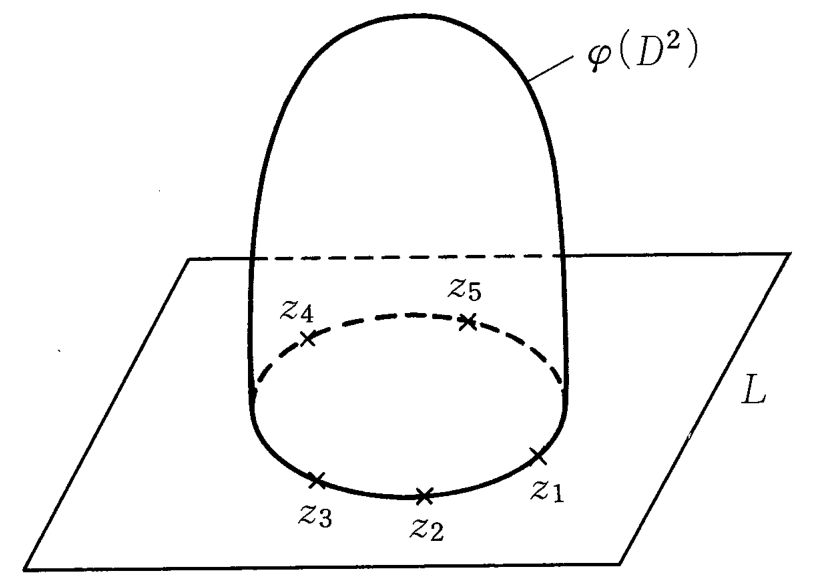
\includegraphics[width=0.48\textwidth]{figures/fig6.19.png}
  \figtitle{6.19}{$\mathcal M_k(M,J_M;L;\beta)$ 的元（原书 p.346）}
\end{figure}

容易看出，定义 6.208 是 §6.2 所述模空间 $\mathcal M_{g,k}(M,J_M;\beta)$ 向有拉格朗日子流形情形的自然推广。

% [原文 p.347]
$\mathcal M_{0,k}(M,J_M;L;\beta)$ 的紧化 $CM_{0,k}(M,J_M;L;\beta)$ 可与 $CM_{g,k}(M,J_M;\beta)$ 同样地构成。$CM_{0,k}(M,J_M;L;\beta)$ 的元，例如由图 6.20 表示。紧化的准确定义省略。

\begin{figure}[htbp]
  \centering
  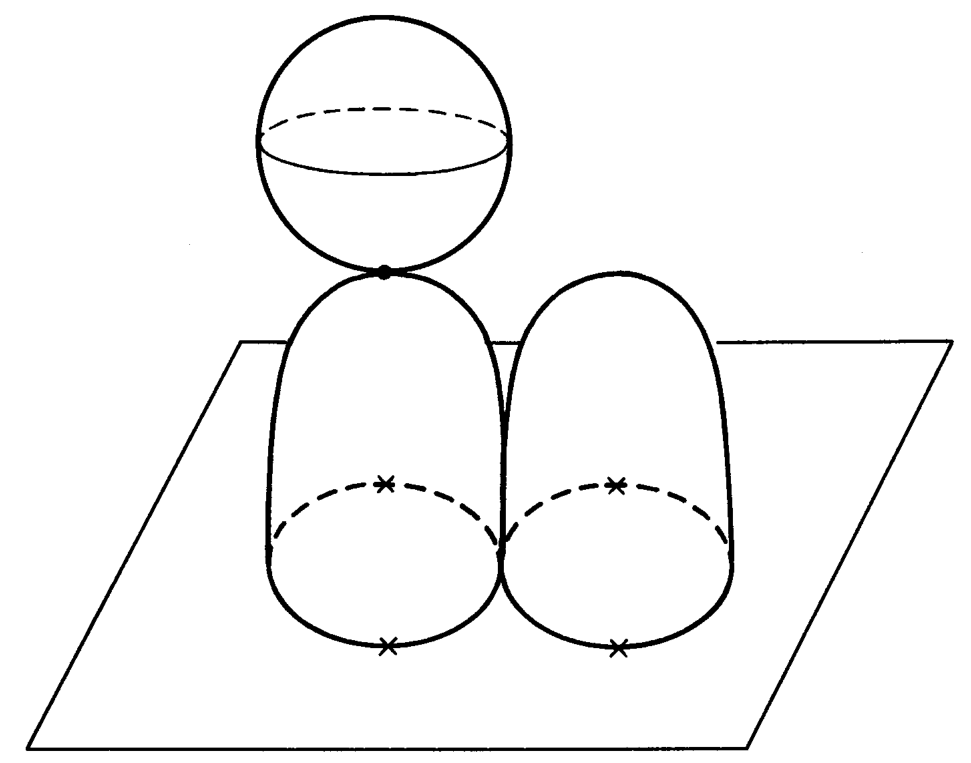
\includegraphics[width=0.55\textwidth]{figures/fig6.20.png}
  \figtitle{6.20}{$CM_{0,k}(M,J_M;L;\beta)$ 的紧化（原书 p.347）}
\end{figure}

设 $\mu(\beta)$ 为 $\beta$ 的 Maslov 指数。若 $L$ 可定向，则 $\mu(\beta)$ 总是偶数（由图表 (4.34) 的可交换性）。

\textbf{假定理 6.209}\quad $CM_{0,k}(M,J_M;L;\beta)$ 是 $\mu(\beta)+n+k-3$ 维的紧致光滑带边流形。$\mathrm{ev}$ 可延拓为从 $CM_{0,k}(M,J_M;L;\beta)$ 出发的光滑映射。
% [Tutor Note: 原书把 6.209 标为「嘘定理」（假定理），意思是：如定理 6.28 一样，它作为字面陈述并不成立，必须代之以虚拟基本类（virtual fundamental class）的定式化；作者用这个称呼提醒读者不要照字面使用。]

与假定理 6.28 同样，假定理 6.209 也按原样并不正确。正确的定式化与 6.28 的情形（见 [124]）相同。维数的计算是定理 4.162。即定理 4.162 表明 $\widetilde M_{0,0}(M,J_M;L;\beta)$ 的虚拟维数是 $\mu(\beta)+n$。因 $\partial D^2$ 上有 $k$ 个点，维数增加 $k$，又因 $PSL(2;\R)$ 的作用减少 $3$，故为 $\mu(\beta)+n+k-3$。

\begin{remark}{6.210}
  注意假定理 6.209 的陈述中，说 $CM_{0,k}(M,J_M;L;\beta)$ 是“带角”流形。这是与 Gromov–Witten 不变量的情形的一大差别。带角流形上没有基本同调类。这就是观察 6.206 (1) 的理由。如例 6.211 所示，角与边界实际会出现。
\end{remark}
% [Tutor Note: 带角流形（manifold with corners）。它与带边流形的区别是：边界本身又带边界，故基本同调类不能直接定义。GW 理论中靠虚拟基本类绕过这一点，这里则是弱 $A_{\infty}$ 结构出现的根源。]

% [原文 p.348]
\begin{example}{6.211}
  设 $M$ 为一点，考虑 $CM_{0,4}(M,J_M;L;0)$。（即不考虑映射，只考虑 $(z_1,z_2,z_3,z_4)\in\partial D^2$。）这个空间显然同胚于闭区间，两个边界对应下面的图 6.21。
\end{example}

\begin{figure}[htbp]
  \centering
  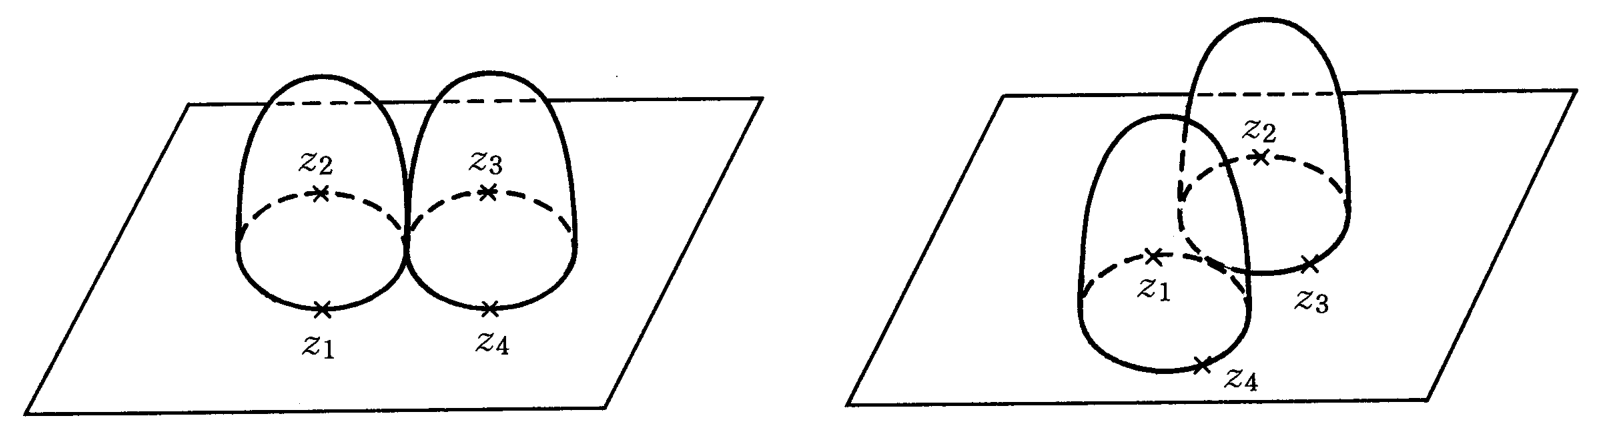
\includegraphics[width=0.82\textwidth]{figures/fig6.21.png}
  \figtitle{6.21}{对应边界的元（原书 p.348）}
\end{figure}

\begin{assumption}{6.212}
  存在 $\tilde w_2\in H^2(M;\Z_2)$，使 $\tilde w_2$ 到 $H^2(L;\Z_2)$ 的拉回与 $L$ 的第 2 Stiefel–Whitney 类一致。又给 $L$ 定向。
\end{assumption}
% [Tutor Note: 原书从 p.348 起把这个类时而印作 $\tilde w_2$、时而印作 $\tilde w^2$（后者易误读为平方），这里统一按 $\tilde w_2$ 处理；它到 $L$ 的拉回等于 $w_2(L)$，是 $L$ 可定向且 $CM_{0,k}$ 可定向的拓扑条件。]

\begin{theorem}{6.213}
  设假定 6.212 成立，并确定 $\tilde w_2$ 与 $L$ 的定向。则 $CM_{0,k}(M,J_M;L;\beta)$ 的定向被确定。
\end{theorem}

如 §4.4 末尾所注意的，定理 6.213 用定理 4.162 的族的指数版证明。证明省略。以后固定 $\tilde w_2\in H^2(M;\Z_2)$，只考虑满足假定 6.212 的带定向拉格朗日子流形。同时考虑两个以上拉格朗日子流形 $L_i$ 时，设 $w_2(L_i)$ 是同一 $\tilde w_2$ 的限制。

现在，设 $x_i=(P_i,\psi_i)$，$i=1,\dots,k$ 为 $L$ 的几何链。

\begin{definition}{6.214}
  对 $k=0,1,\dots$、$\beta\neq0$，令
  \[
    \mathrm{m}_{k,\beta}(x_1,\dots,x_k)=\left((P_1\times\dots\times P_k)\times_{\mathrm{ev}_1,\dots,\mathrm{ev}_k}CM_{0,k+1}(M,J_M;L;\beta),\mathrm{ev}_{k+1}\right).
  \]
  又当 $\beta=0$ 时，令 $\mathrm{m}_{k,0}(P,\psi)=(\partial P,\psi)$（普通的边界作用素），且 $k\neq1$ 时 $\mathrm{m}_{k,0}=0$。把它们相加，由下式定义 $\mathrm{m}_k$：
  \begin{equation}
    \mathrm{m}_k=\sum_\beta\mathrm{m}_{k,\beta}T^{\beta\cap[\omega]}\otimes u^{\mu(\beta)/2}. \tag{6.70}
  \end{equation}
\end{definition}

在定义 6.214 中，必须对几何链加上为定义纤维积所需的横截正则性假定。关于这一点省略。(6.70) 的右边成为 $\Lambda_{nov,\Q}$ 系数的几何链，这可以...

% [原文 p.349]
与 Gromov–Witten 不变量的情形同样，用紧致性定理（引理 6.49 的类似物）证明。

下一定理是 [122] 的主定理。设 $C_*(L;\Z)$ 为 $L$ 的几何链所作链复体的可算部分复体。用 $C^*(L;\Z)=C_{n-*}(L;\Z)$ 把它改成余链复体。令 $C^*(L;\Lambda_{nov,\Q})=C^*(L;\Z)\otimes\Lambda_{nov,\Q}$。

\begin{theorem}{6.215}
  $\mathrm{m}$ 们在 $\mathrm{II}C^*(L;\Lambda_{nov,\Q})$ 上确定滤过弱 $A_{\infty}$ 代数的结构。这个滤过弱 $A_{\infty}$ 代数是决定 $L$ 的有理同伦型的 $A_{\infty}$ 代数的形变。

  弱 $A_{\infty}$ 代数的同伦型不依赖近复结构 $J_M$ 等，而由辛流形 $M$ 与拉格朗日子流形 $L$ 决定。

  当 $\psi$ 为完全辛同胚时，$L$ 决定的弱 $A_{\infty}$ 代数与 $\psi(L)$ 决定的弱 $A_{\infty}$ 代数同伦等价。
\end{theorem}
% [Tutor Note: 记号 $\mathrm{II}C^*$ 是原书的写法；由后文 $(\mathrm{II}C)^0(L;\Lambda_{nov,\Q})=C^1(L;\Lambda_{nov,\Q})$ 可知它就是复体 $C^*$ 的次数平移（$\mathrm{II}C^i=C^{i+1}$）。原书这一节把 $A_\infty$ 印作 $A_{\infty}$（无穷在右上角），译文照原书。]

证明的想法与 Gromov–Witten 不变量的构成及结合律的证明十分相似。即考察带点黎曼面的退化。不同的是 $CM_{0,k+1}(M,J_M;L;\beta)$ 带边界。不能叙述证明的细节，但说明概要。应证明的弱 $A_{\infty}$ 结构的关系式是
\begin{equation}
  \sum_{k_1+k_2=k+1}\sum_{\beta_1+\beta_2=\beta}\pm\mathrm{m}_{k_1,\beta_1}(x_1,\dots,x_i,\mathrm{m}_{k_2,\beta_2}(x_{i+1},\dots,x_{i+m_2}),x_{i+m_2+1},\dots,x_k)=0 \tag{6.71}
\end{equation}
（关于符号的考察微妙而重要，但省略。）$\beta_1=0$、$k_1=1$ 时 (6.71) 的项可表为
\begin{equation}
  \partial\mathrm{m}_{k,\beta}(x_1,\dots,x_k). \tag{6.72}
\end{equation}
设 $x_i=(P_i,\psi_i)$，则 (6.72) 是定义 6.214 的几何链的边界。定义 6.214 的几何链的边界，与由裂成两个的圆盘出发的伪全纯映射的模空间一致。设裂开的两个圆盘为 $D_1$ 与 $D_2$，$\varphi_1:(D_1,\partial D_1)\to M$、$\varphi_2:(D_2,\partial D_2)\to M$ 为伪全纯映射。带名点 $z_i$ 乘在 $\partial D_1,\partial D_2$ 之一上。$z_i,\dots,z_{i+m_1}\in\partial D_2$、其余乘在 $\partial D_1$ 上，且 $\varphi_1,\varphi_2$ 的同调类为 $\beta_1,\beta_2$ 的情形所对应者，就是 (6.71) 中与这个 $k_1,k_2,\beta_1,\beta_2$ 对应的项（图 6.22）。写成式子就是

\begin{figure}[htbp]
  \centering
  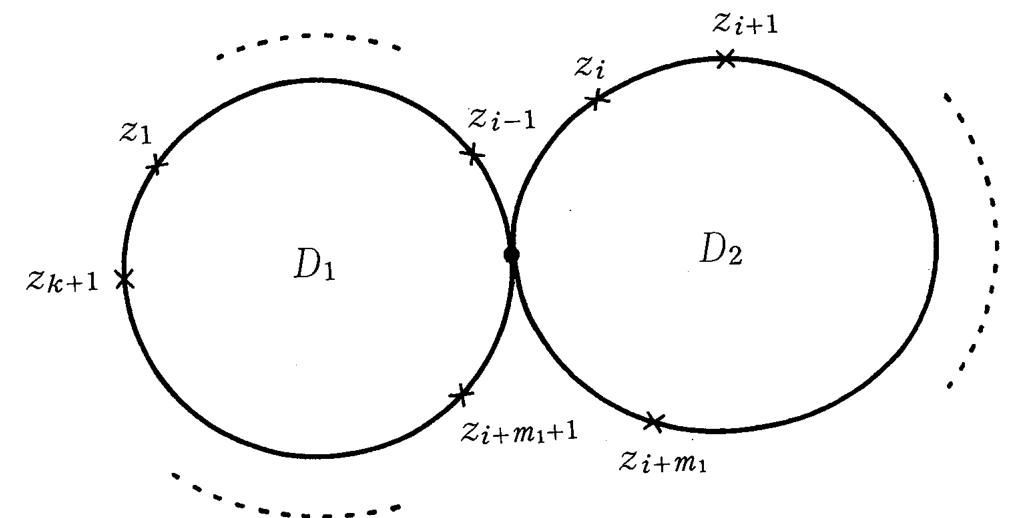
\includegraphics[width=0.58\textwidth]{figures/fig6.22.png}
  \figtitle{6.22}{裂开的圆盘（原书 p.350）}
\end{figure}

% [原文 p.350]
下面这样。
\[
  \resizebox{0.97\linewidth}{!}{$\begin{aligned} &\partial\left((P_1\times\dots\times P_k)\times_{\mathrm{ev}_1,\dots,\mathrm{ev}_k}CM_{0,k+1}(M,J_M;L;\beta)\right)\\ &\quad=\sum_i\pm(P_1\times\dots\partial P_i\cdots\times P_k)\times_{\mathrm{ev}_1,\dots,\mathrm{ev}_k}CM_{0,k+1}(M,J_M;L;\beta)\\ &\quad+\sum_{\beta_1+\beta_2=\beta}\sum_{1\le i\le j\le k}\pm\Bigl(P_1\times\dots\times P_{i-1}\times\bigl((P_i\times\dots\times P_j)\times_{\mathrm{ev}}CM_{0,j-i}(M,J_M;L;\beta_1)\bigr)\\ &\qquad\qquad\times(P_{j+1}\times\dots\times P_k)\times_{\mathrm{ev}}CM_{0,k-j+i}(M,J_M;L;\beta_2)\Bigr). \end{aligned}$}
\]

\begin{remark}{6.216}
  在 $C^*(L;\Z)$ 上，以 $\mathrm{m}_2(P,Q)=P\cap Q$ 为积的微分多元环的结构大致确定。说“大致”，是因为对 $P\cap P$ 横截正则性绝不成立。这在有理同伦论（[310], [351]\footnote{易读的解说书是 [157]。不过 [157] 完全没有叙述形变理论这一重要侧面。}）中是重大问题。Sullivan 用某种微分形式所作有限生成微分多元环解决了这一困难。不是在微分形式、而是在奇异同调（几何链的同调本质上是一种奇异同调）的立场上解决这一困难，需要把范围扩大到 $A_{\infty}$ 代数来考虑。定理 6.215 中所述“决定有理同伦型的 $A_{\infty}$ 代数”，就是指这样得到的（量子修正前的）$A_{\infty}$ 代数。
\end{remark}

\begin{remark}{6.217}
  在 Floer 同调上考虑 $A_{\infty}$ 结构始于 [114]。它与镜像对称的关系由 [215], [219] 发现。对勒让德结，Chekanov [60] 发现的 $A_{\infty}$ 代数也与定理 6.215 的 $A_{\infty}$ 代数有深刻关系。
\end{remark}

% [原文 p.351]
定理 6.215 得到的是弱 $A_{\infty}$ 代数，不是 $A_{\infty}$ 代数。因此 $\mathrm{m}_1\mathrm{m}_1=0$ 一般不成立。弱 $A_{\infty}$ 代数情形，(6.41) 代之以
\[
  \mathrm{m}_1\mathrm{m}_1(x)+\mathrm{m}_2(c,x)+\mathrm{m}_2(x,c)=0.
\]
这里令 $c=\mathrm{m}_0(1)$。这就是观察 6.206 (1) 的说明\footnote{这里的说明是抽象的，更具体的说明见 [122], [290] 等。}。解决这个问题的处方已在 §6.4 说明。即考虑满足方程式 (6.51) 的 $b\in(\mathrm{II}C)^0(L;\Lambda_{nov,\Q})=C^1(L;\Lambda_{nov,\Q})$，用 (6.49) 变形 $A_{\infty}$ 结构。$b$ 是 $\mathcal M(L)=\mathcal M(C^*(L;\Lambda_{nov,\Q}))$ 的元。这里右边由定义 6.119 与 6.128 确定。（不过，定义 6.128 的规范等价的定义需要稍作改变。）于是由命题 6.117 得到下面的系。

\begin{corollary}{6.218}
  对 $\mathcal M(L)$ 的元 $[b]$，$A_{\infty}$ 代数被确定。
\end{corollary}

这样就能把 6.182 作为正确的猜想叙述。

\begin{conjecture}{6.219}
  设 $M$ 为辛流形，$M^\dagger$ 为其镜像的复流形。对 $M$ 的使定理 6.215 的弱 $A_{\infty}$ 代数非障碍的拉格朗日子流形 $L$，存在 $M^\dagger$ 的解析凝聚层范畴的导出范畴的对象 $\mathcal F_L$，且 $\mathcal F_L$ 的无穷小形变的（扩大）模空间与 $\mathcal M(L)$ 一致。
\end{conjecture}

\begin{remark}{6.220}
  $\mathcal M(L)$ 的元 $b$ 表为 $b=\sum b_iu^{-i}$（$i=0,1,2,\dots$）。由于 $\deg u=2$，$b_i$ 是 $2i+1$ 次链。$b_0$ 与 1 次上同调有关，故作为拉格朗日子流形形变的参数自然出现。$b=i$，$i=1,\dots$ 没有直接的几何意义。因此，应把 $\mathcal M(L)$ 看作扩大模空间。
\end{remark}

由系 6.218，各个 $[b]\in\mathcal M(L)$ 决定链复体的边界映射 $\mathrm{m}_1^b$。

\begin{definition}{6.221}
  称 $\mathrm{m}_1^b$ 的上同调为 Floer 上同调，写作 $HF((L,b),(L,b))$。
\end{definition}

\begin{theorem*}{6.222}
  存在谱序列 $E_*^*$，使 $E_2^*\simeq H^*(L;\Lambda_{nov,\Q})$，且收敛于 $HF((L,b),(L,b))$。
\end{theorem*}
\begin{proof}
% [原文 p.352]
  考虑能量滤过，取其关于这个滤过的谱序列即可。
\end{proof}

\begin{remark}{6.223}
  定理 6.222 的谱序列，在拉格朗日子流形单调的情形由 Oh [291] 构成，并由 [122] 推广。
\end{remark}

\begin{remark}{6.224}
  要应用于拉格朗日子流形的研究，需要谱序列的微分的更详细性质。这里不叙述，但例如若 $L\to M$ 在同调上诱导单射，则谱序列在 $E_2$ 项退化。
\end{remark}

用系 6.218，对 $\mathcal M(L)$ 的元 $b$ 构成 Frobenius 代数。设 $\langle\cdot,\cdot\rangle:C_*(L;\Lambda_{nov,\Q})\otimes C_*(L;\Lambda_{nov,\Q})\to\Lambda_{nov,\Q}$ 为 Poincaré 对偶。即令
\[
  \langle P_1,P_2\rangle=
  \begin{cases}
    P_1\cap P_2\in H_0(L;\Q)\cong\Q, & \deg P_1+\deg P_2=n \text{ 时},\\
    0, & \deg P_1+\deg P_2\neq0 \text{ 时},
  \end{cases}
\]
并把 $\langle P_1,P_2\rangle$ 作 $\Lambda_{nov,\Q}$ 线性扩张。
% [Tutor Note: 原书第二个分支印作「$\deg P_1+\deg P_2\neq0$ 时」，按 Poincaré 对偶的定义应为「$\neq n$ 时」（否则 $\deg P_1+\deg P_2=n=0$ 的平凡情形会漏掉）。]

\begin{lemma*}{6.225}
  \[
    \langle\mathrm{m}_k(x_1\cdots x_k),x_{k+1}\rangle=(-1)^{x_{k+1}(x_1+\dots+x_k)}\langle\mathrm{m}_k(x_{k+1}x_1\cdots x_{k-1}),x_k\rangle.
  \]
  这里 $-1$ 的肩表示移动之后的次数。
\end{lemma*}
\begin{proof}
  设 $x_i=(P_i,\psi_i)$，则两边（除符号外）由下列几何链表示。
  \[
    \sum_\beta(P_1\times\dots\times P_{k+1})\cap\mathrm{ev}_*(CM_{0,k+1}(M,J_M;L;\beta))T^{\beta\cap[\omega]}\otimes u^{\mu(\beta)/2}.
  \]
  这里 $\cap$ 是 $L^{k+1}$ 中的相交形式。上式中的项，若 $\sum(n-\dim P_i)=\dim CM_{0,k+1}(M,J_M;L;\beta)$ 不成立，则视为 $0$。
\end{proof}

由引理 6.225 与系 6.218，在 $HF((L,b),(L,b))$ 上确定 Frobenius 代数结构 $\langle\cdot,\cdot\rangle$、$\mathrm{m}_2^b$。

定义 6.221 中只定义了同一拉格朗日子流形之间的 Floer 同调，但两个不同拉格朗日子流形之间的 Floer 同调也可定义。为此，需要把普遍 Novikov 环稍微放大，考虑
\[
  \Lambda_{nov,+,\Q}=\Lambda'_{nov,+,\Q}\otimes_\Q\Q[u,u^{-1}]
\]
这一边。（$\Lambda'_{nov,+,\Q}$ 在 §5.44 中定义。）

% CHUNK ch06d2 DONE

